\section{UNet}
The typical use of CNNs was mainly classification. The original architectures would usually just recognise what is on the image, but not where - which is the point of segmentation. In 2015, a new type of network for segmentation of biomedical images Unet was introduced \cite{unet2015}.

It is a FCV - fully convolutional network. That means there are no dense layers, only convolutions. This architecture (\ref{fig:unet}) consists of two parts or paths - \textbf{encoder} and \textbf{decoder}, which resembles the letter U. Hence, the name U-Net. Encoder serves for down sampling the high-resolution input image to a low-resolution output to find out what is in the image. Decoder up samples the low-resolution image back to the original resolution, retrieving locations of the features.

\begin{figure}[ht!]
    \centering
    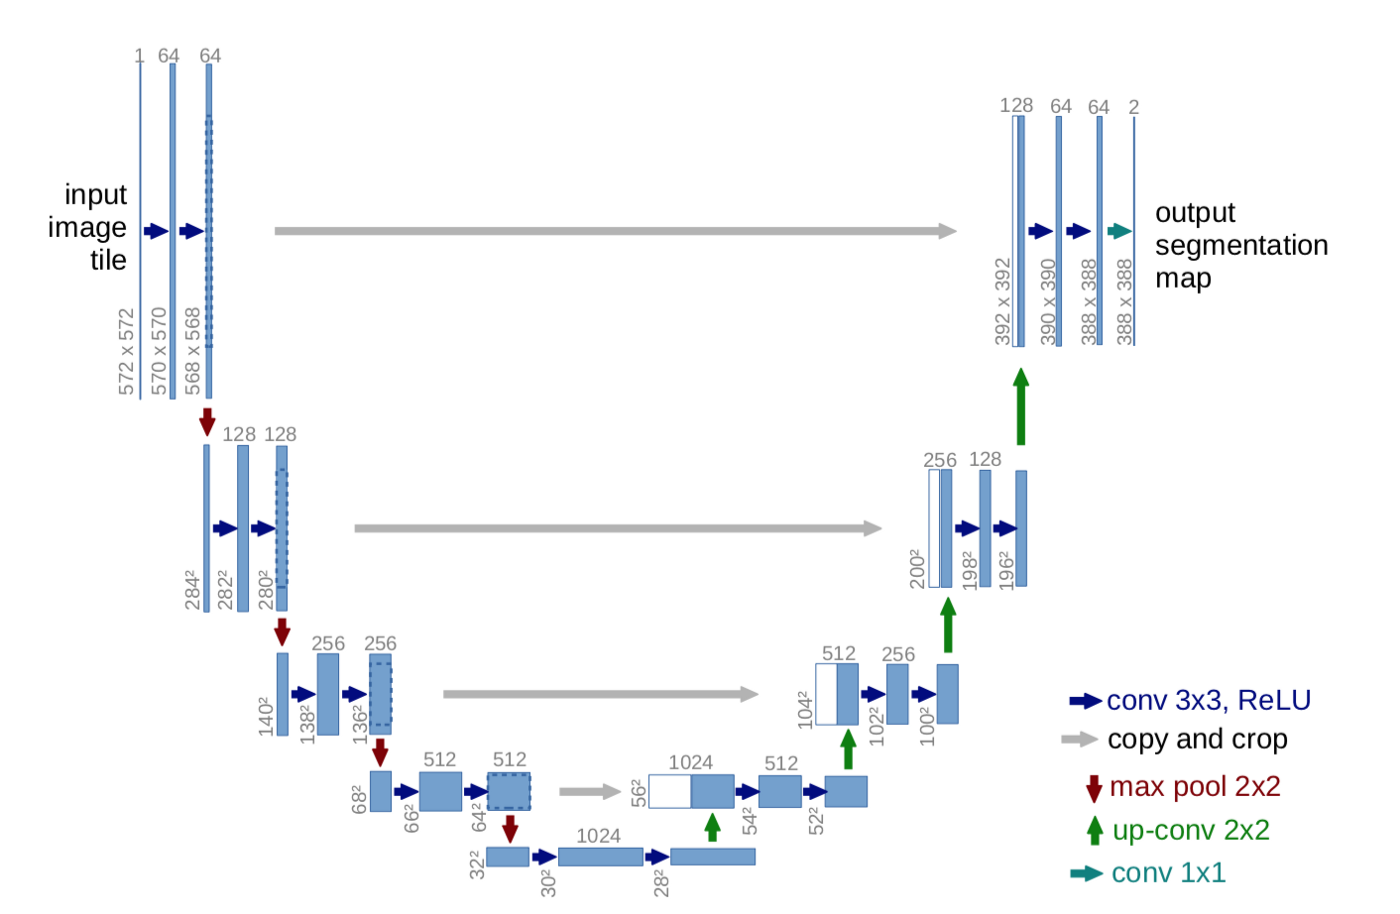
\includegraphics[width=300pt]{images/unet.png}
    \caption[Architecture of UNet]{Architecture of UNet \cite{unet2015}}
    \label{fig:unet}
\end{figure}

Encoder is a typical CNN, consisting of 3 blocks containing 2 convolutional layers followed by a max-pooling layer.

Decoder is more interesting. It is symmetrical to the encoder - 3 block consisting of up-convolution (transposed convolution) and 2 convolutions. The output is a predicted segmentation mask. Transposed convolution can be viewed as an operation opposite to convolution (but it is not the most precise definition). It creates a higher-resolution image from a low-resolution image. Furthermore, every result of up-convolution is concatenated with the feature map from the corresponding level in the encoder through skip connections. UNet has proven to perform very well on biomedical images.  

\pagebreak